% Created by tikzDevice version 0.12.6 on 2026-06-17 14:28:33
% !TEX encoding = UTF-8 Unicode
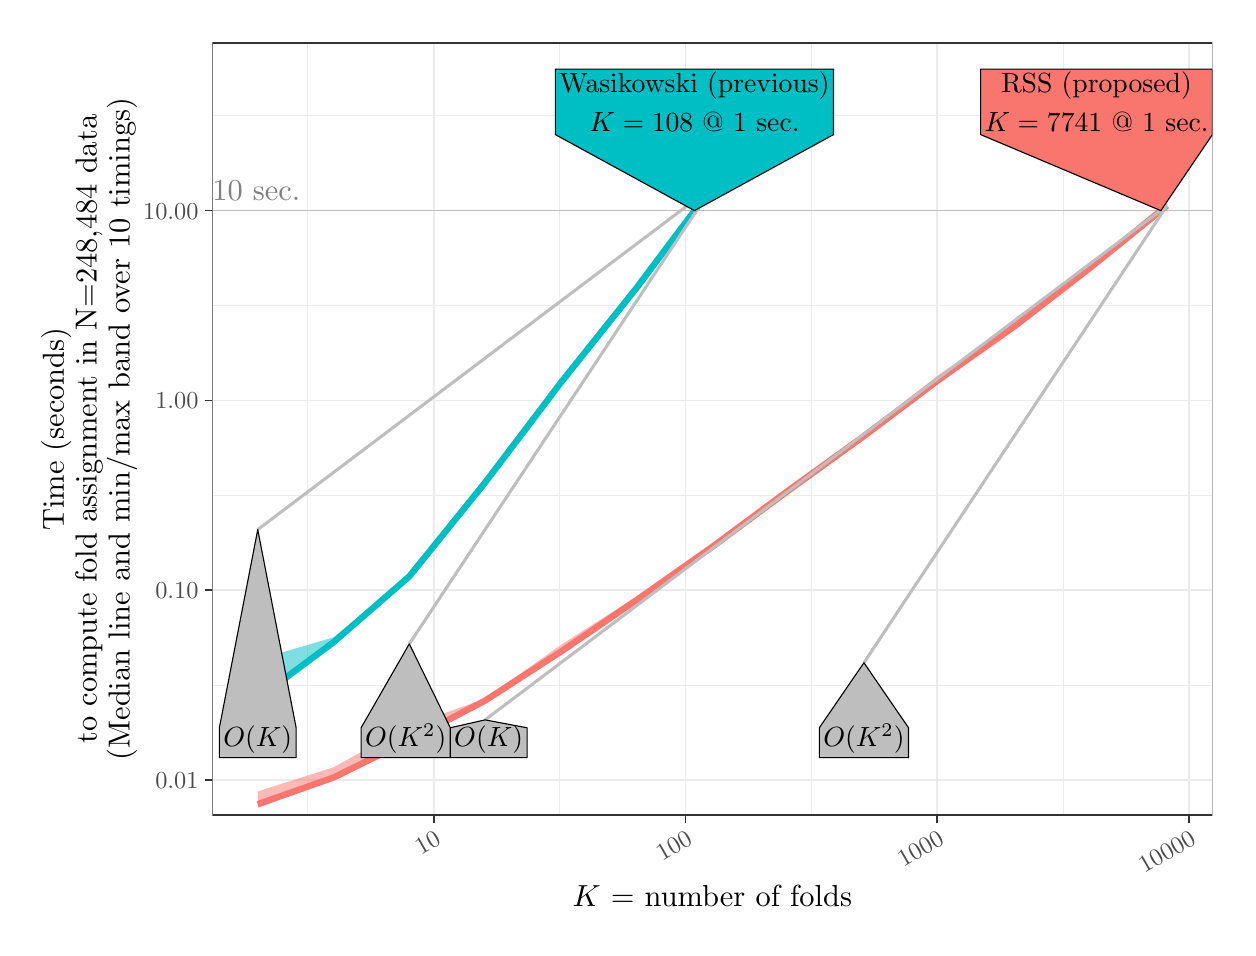
\begin{tikzpicture}[x=1pt,y=1pt]
\definecolor{fillColor}{RGB}{255,255,255}
\path[use as bounding box,fill=fillColor,fill opacity=0.00] (0,0) rectangle (433.62,325.21);
\begin{scope}
\path[clip] (  0.00,  0.00) rectangle (433.62,325.21);
\definecolor{drawColor}{RGB}{255,255,255}
\definecolor{fillColor}{RGB}{255,255,255}

\path[draw=drawColor,line width= 0.6pt,line join=round,line cap=round,fill=fillColor] (  0.00,  0.00) rectangle (433.62,325.21);
\end{scope}
\begin{scope}
\path[clip] ( 66.71, 40.64) rectangle (428.12,319.71);
\definecolor{fillColor}{RGB}{255,255,255}

\path[fill=fillColor] ( 66.71, 40.64) rectangle (428.12,319.71);
\definecolor{drawColor}{gray}{0.92}

\path[draw=drawColor,line width= 0.3pt,line join=round] ( 66.71, 87.62) --
	(428.12, 87.62);

\path[draw=drawColor,line width= 0.3pt,line join=round] ( 66.71,156.21) --
	(428.12,156.21);

\path[draw=drawColor,line width= 0.3pt,line join=round] ( 66.71,224.80) --
	(428.12,224.80);

\path[draw=drawColor,line width= 0.3pt,line join=round] ( 66.71,293.38) --
	(428.12,293.38);

\path[draw=drawColor,line width= 0.3pt,line join=round] (101.24, 40.64) --
	(101.24,319.71);

\path[draw=drawColor,line width= 0.3pt,line join=round] (192.19, 40.64) --
	(192.19,319.71);

\path[draw=drawColor,line width= 0.3pt,line join=round] (283.14, 40.64) --
	(283.14,319.71);

\path[draw=drawColor,line width= 0.3pt,line join=round] (374.09, 40.64) --
	(374.09,319.71);

\path[draw=drawColor,line width= 0.6pt,line join=round] ( 66.71, 53.33) --
	(428.12, 53.33);

\path[draw=drawColor,line width= 0.6pt,line join=round] ( 66.71,121.91) --
	(428.12,121.91);

\path[draw=drawColor,line width= 0.6pt,line join=round] ( 66.71,190.50) --
	(428.12,190.50);

\path[draw=drawColor,line width= 0.6pt,line join=round] ( 66.71,259.09) --
	(428.12,259.09);

\path[draw=drawColor,line width= 0.6pt,line join=round] (146.71, 40.64) --
	(146.71,319.71);

\path[draw=drawColor,line width= 0.6pt,line join=round] (237.67, 40.64) --
	(237.67,319.71);

\path[draw=drawColor,line width= 0.6pt,line join=round] (328.62, 40.64) --
	(328.62,319.71);

\path[draw=drawColor,line width= 0.6pt,line join=round] (419.57, 40.64) --
	(419.57,319.71);
\definecolor{drawColor}{gray}{0.50}

\node[text=drawColor,anchor=base west,inner sep=0pt, outer sep=0pt, scale=  1.10] at ( 66.71,262.88) { 10 sec.};
\definecolor{drawColor}{RGB}{190,190,190}

\path[draw=drawColor,line width= 0.6pt,line join=round] ( 66.71,259.09) -- (428.12,259.09);
\definecolor{fillColor}{RGB}{248,118,109}

\path[fill=fillColor,fill opacity=0.50] ( 83.14, 49.23) --
	(110.52, 57.94) --
	(137.90, 73.01) --
	(165.28, 82.72) --
	(192.66,102.15) --
	(220.04,119.69) --
	(247.42,138.58) --
	(274.80,158.71) --
	(302.18,178.64) --
	(329.55,200.00) --
	(356.93,218.66) --
	(384.31,239.01) --
	(411.69,261.83) --
	(411.69,260.23) --
	(384.31,237.76) --
	(356.93,216.81) --
	(329.55,197.65) --
	(302.18,177.17) --
	(274.80,156.60) --
	(247.42,137.06) --
	(220.04,117.58) --
	(192.66, 99.05) --
	(165.28, 81.55) --
	(137.90, 67.33) --
	(110.52, 53.80) --
	( 83.14, 43.29) --
	cycle;

\path[] ( 83.14, 49.23) --
	(110.52, 57.94) --
	(137.90, 73.01) --
	(165.28, 82.72) --
	(192.66,102.15) --
	(220.04,119.69) --
	(247.42,138.58) --
	(274.80,158.71) --
	(302.18,178.64) --
	(329.55,200.00) --
	(356.93,218.66) --
	(384.31,239.01) --
	(411.69,261.83);

\path[] (411.69,260.23) --
	(384.31,237.76) --
	(356.93,216.81) --
	(329.55,197.65) --
	(302.18,177.17) --
	(274.80,156.60) --
	(247.42,137.06) --
	(220.04,117.58) --
	(192.66, 99.05) --
	(165.28, 81.55) --
	(137.90, 67.33) --
	(110.52, 53.80) --
	( 83.14, 43.29);
\definecolor{fillColor}{RGB}{0,191,196}

\path[fill=fillColor,fill opacity=0.50] ( 83.14, 96.87) --
	(110.52,104.91) --
	(137.90,127.24) --
	(165.28,161.72) --
	(192.66,197.57) --
	(220.04,231.73) --
	(247.42,268.22) --
	(247.42,267.07) --
	(220.04,230.59) --
	(192.66,196.24) --
	(165.28,160.23) --
	(137.90,126.33) --
	(110.52,102.44) --
	( 83.14, 82.18) --
	cycle;

\path[] ( 83.14, 96.87) --
	(110.52,104.91) --
	(137.90,127.24) --
	(165.28,161.72) --
	(192.66,197.57) --
	(220.04,231.73) --
	(247.42,268.22);

\path[] (247.42,267.07) --
	(220.04,230.59) --
	(192.66,196.24) --
	(165.28,160.23) --
	(137.90,126.33) --
	(110.52,102.44) --
	( 83.14, 82.18);
\definecolor{drawColor}{RGB}{248,118,109}

\path[draw=drawColor,line width= 2.3pt,line join=round] ( 83.14, 44.61) --
	(110.52, 54.25) --
	(137.90, 67.71) --
	(165.28, 82.04) --
	(192.66, 99.73) --
	(220.04,118.37) --
	(247.42,137.63) --
	(274.80,157.90) --
	(302.18,177.62) --
	(329.55,198.20) --
	(356.93,217.54) --
	(384.31,238.73) --
	(411.69,260.90);
\definecolor{drawColor}{RGB}{0,191,196}

\path[draw=drawColor,line width= 2.3pt,line join=round] ( 83.14, 82.75) --
	(110.52,103.14) --
	(137.90,126.92) --
	(165.28,160.83) --
	(192.66,196.94) --
	(220.04,231.21) --
	(247.42,267.72);
\definecolor{drawColor}{RGB}{190,190,190}

\path[draw=drawColor,line width= 1.1pt,line join=round] (165.28, 75.08) --
	(192.66, 95.72) --
	(220.04,116.37) --
	(247.42,137.02) --
	(274.80,157.67) --
	(302.18,178.31) --
	(329.55,198.96) --
	(356.93,219.61) --
	(384.31,240.25) --
	(411.69,260.90);

\path[draw=drawColor,line width= 1.1pt,line join=round] (302.18, 95.72) --
	(329.55,137.02) --
	(356.93,178.31) --
	(384.31,219.61) --
	(411.69,260.90);

\path[draw=drawColor,line width= 1.1pt,line join=round] ( 83.14,143.84) --
	(110.52,164.49) --
	(137.90,185.14) --
	(165.28,205.78) --
	(192.66,226.43) --
	(220.04,247.08) --
	(247.42,267.72);

\path[draw=drawColor,line width= 1.1pt,line join=round] (137.90,102.55) --
	(165.28,143.84) --
	(192.66,185.14) --
	(220.04,226.43) --
	(247.42,267.72);
\end{scope}
\begin{scope}
\path[clip] ( 66.71, 40.64) rectangle (428.12,319.71);
\definecolor{drawColor}{RGB}{0,0,0}
\definecolor{fillColor}{RGB}{248,118,109}

\path[draw=drawColor,line width= 0.4pt,line join=round,line cap=round,fill=fillColor] (344.35,310.25) --
	(428.12,310.25) --
	(428.12,286.57) --
	(409.46,259.09) --
	(344.35,286.57) --
	cycle;
\definecolor{fillColor}{RGB}{0,191,196}

\path[draw=drawColor,line width= 0.4pt,line join=round,line cap=round,fill=fillColor] (190.68,310.25) --
	(291.20,310.25) --
	(291.20,286.57) --
	(240.94,259.09) --
	(190.68,286.57) --
	cycle;

\node[text=drawColor,anchor=base,inner sep=0pt, outer sep=0pt, scale=  1.00] at (386.24,301.94) {RSS (proposed)};

\node[text=drawColor,anchor=base,inner sep=0pt, outer sep=0pt, scale=  1.00] at (386.24,287.54) {$K=7741$ @ 1 sec.};

\node[text=drawColor,anchor=base,inner sep=0pt, outer sep=0pt, scale=  1.00] at (240.94,301.94) {Wasikowski (previous)};

\node[text=drawColor,anchor=base,inner sep=0pt, outer sep=0pt, scale=  1.00] at (240.94,287.54) {$K=108$ @ 1 sec.};
\end{scope}
\begin{scope}
\path[clip] ( 66.71, 40.64) rectangle (428.12,319.71);
\definecolor{drawColor}{RGB}{0,0,0}
\definecolor{fillColor}{RGB}{190,190,190}

\path[draw=drawColor,line width= 0.4pt,line join=round,line cap=round,fill=fillColor] (152.71, 72.23) --
	(165.28, 75.08) --
	(180.45, 72.23) --
	(180.45, 61.42) --
	(152.71, 61.42) --
	cycle;

\path[draw=drawColor,line width= 0.4pt,line join=round,line cap=round,fill=fillColor] ( 69.27, 72.23) --
	( 83.14,143.84) --
	( 97.01, 72.23) --
	( 97.01, 61.42) --
	( 69.27, 61.42) --
	cycle;

\path[draw=drawColor,line width= 0.4pt,line join=round,line cap=round,fill=fillColor] (286.06, 72.23) --
	(302.18, 95.72) --
	(318.29, 72.23) --
	(318.29, 61.42) --
	(286.06, 61.42) --
	cycle;

\path[draw=drawColor,line width= 0.4pt,line join=round,line cap=round,fill=fillColor] (120.49, 72.23) --
	(137.90,102.55) --
	(152.71, 72.23) --
	(152.71, 61.42) --
	(120.49, 61.42) --
	cycle;

\node[text=drawColor,anchor=base,inner sep=0pt, outer sep=0pt, scale=  1.00] at (166.58, 65.35) {$O(K)$};

\node[text=drawColor,anchor=base,inner sep=0pt, outer sep=0pt, scale=  1.00] at ( 83.14, 65.35) {$O(K)$};

\node[text=drawColor,anchor=base,inner sep=0pt, outer sep=0pt, scale=  1.00] at (302.18, 65.35) {$O(K^2)$};

\node[text=drawColor,anchor=base,inner sep=0pt, outer sep=0pt, scale=  1.00] at (136.60, 65.35) {$O(K^2)$};
\definecolor{drawColor}{gray}{0.20}

\path[draw=drawColor,line width= 0.6pt,line join=round,line cap=round] ( 66.71, 40.64) rectangle (428.12,319.71);
\end{scope}
\begin{scope}
\path[clip] (  0.00,  0.00) rectangle (433.62,325.21);
\definecolor{drawColor}{gray}{0.30}

\node[text=drawColor,anchor=base east,inner sep=0pt, outer sep=0pt, scale=  0.88] at ( 61.76, 50.30) {0.01};

\node[text=drawColor,anchor=base east,inner sep=0pt, outer sep=0pt, scale=  0.88] at ( 61.76,118.88) {0.10};

\node[text=drawColor,anchor=base east,inner sep=0pt, outer sep=0pt, scale=  0.88] at ( 61.76,187.47) {1.00};

\node[text=drawColor,anchor=base east,inner sep=0pt, outer sep=0pt, scale=  0.88] at ( 61.76,256.06) {10.00};
\end{scope}
\begin{scope}
\path[clip] (  0.00,  0.00) rectangle (433.62,325.21);
\definecolor{drawColor}{gray}{0.20}

\path[draw=drawColor,line width= 0.6pt,line join=round] ( 63.96, 53.33) --
	( 66.71, 53.33);

\path[draw=drawColor,line width= 0.6pt,line join=round] ( 63.96,121.91) --
	( 66.71,121.91);

\path[draw=drawColor,line width= 0.6pt,line join=round] ( 63.96,190.50) --
	( 66.71,190.50);

\path[draw=drawColor,line width= 0.6pt,line join=round] ( 63.96,259.09) --
	( 66.71,259.09);
\end{scope}
\begin{scope}
\path[clip] (  0.00,  0.00) rectangle (433.62,325.21);
\definecolor{drawColor}{gray}{0.20}

\path[draw=drawColor,line width= 0.6pt,line join=round] (146.71, 37.89) --
	(146.71, 40.64);

\path[draw=drawColor,line width= 0.6pt,line join=round] (237.67, 37.89) --
	(237.67, 40.64);

\path[draw=drawColor,line width= 0.6pt,line join=round] (328.62, 37.89) --
	(328.62, 40.64);

\path[draw=drawColor,line width= 0.6pt,line join=round] (419.57, 37.89) --
	(419.57, 40.64);
\end{scope}
\begin{scope}
\path[clip] (  0.00,  0.00) rectangle (433.62,325.21);
\definecolor{drawColor}{gray}{0.30}

\node[text=drawColor,rotate= 30.00,anchor=base east,inner sep=0pt, outer sep=0pt, scale=  0.88] at (149.74, 30.44) {10};

\node[text=drawColor,rotate= 30.00,anchor=base east,inner sep=0pt, outer sep=0pt, scale=  0.88] at (240.70, 30.44) {100};

\node[text=drawColor,rotate= 30.00,anchor=base east,inner sep=0pt, outer sep=0pt, scale=  0.88] at (331.65, 30.44) {1000};

\node[text=drawColor,rotate= 30.00,anchor=base east,inner sep=0pt, outer sep=0pt, scale=  0.88] at (422.60, 30.44) {10000};
\end{scope}
\begin{scope}
\path[clip] (  0.00,  0.00) rectangle (433.62,325.21);
\definecolor{drawColor}{RGB}{0,0,0}

\node[text=drawColor,anchor=base,inner sep=0pt, outer sep=0pt, scale=  1.10] at (247.42,  7.64) {$K$ = number of folds};
\end{scope}
\begin{scope}
\path[clip] (  0.00,  0.00) rectangle (433.62,325.21);
\definecolor{drawColor}{RGB}{0,0,0}

\node[text=drawColor,rotate= 90.00,anchor=base,inner sep=0pt, outer sep=0pt, scale=  1.10] at ( 13.08,180.18) {Time (seconds)};

\node[text=drawColor,rotate= 90.00,anchor=base,inner sep=0pt, outer sep=0pt, scale=  1.10] at ( 24.96,180.18) {to compute fold assignment in N=248,484 data};

\node[text=drawColor,rotate= 90.00,anchor=base,inner sep=0pt, outer sep=0pt, scale=  1.10] at ( 36.84,180.18) {(Median line and min/max band over 10 timings)};
\end{scope}
\end{tikzpicture}
